\chapter{Background and Problem Definition}
\label{chap:backgroud}
\adjustmtc
\minitoc

Our contributions bridge standard \ai paradigms and developmental psychology to investigate two fundamental research questions  (1) the language acquisition problem (self-organisation of cultural conventions) and (2) the open-ended skill acquisition problem (self-organisation of trajectories). In this chapter, we will first present standard \ai problems and their associated families of algorithmic solutions before getting into the specifications of the two problems we investigate.

\section{Background: Standard \ai Paradigms}



\subsection{Reinforcement Learning}

\paragraph{Problem}

In a reinforcement learning (\rl) problem, the agent learns to perform sequences of actions in an environment so as to maximize some notion of cumulative reward~\citep{sutton2018reinforcement}. \rl problems are commonly framed as Markov Decision Processes (\mdps): $\m{M}\,=\,\{\m{S},\,\m{A},\,\m{T},\,\rho_0,\,R\}$~\citep{sutton2018reinforcement}. The agent and its environment, as well as their interaction dynamics are defined by the first components $\{\m{S},\,\m{A},\,\m{T},\,\rho_0\}$, where $s\in\m{S}$ describes the current state of the agent-environment interaction and $\rho_0$ is the distribution over initial states. The agent can interact with the environment through actions $a\in\m{A}$. Finally, the dynamics are characterized by the transition function $\m{T}$ that dictates the distribution of the next state $s'$ from the current state and action $\m{T} (s'\mid s,\,a)$. 

The objective of the agent in this environment is defined by the remaining component of the \mdp: $R$. $R$ is the reward function, it computes a reward for any transition: $R(s,\,a,\,s')$. Note that, in a traditional \rl problem, the agent only receives the rewards corresponding to the transitions it experiences but does not have access to the function itself. The objective of the agent is to maximize the cumulative reward computed over complete episodes. When computing the aggregation of rewards, we often introduce discounting and give smaller weights to delayed rewards. $R^\text{tot}_t$ is then computed as $R^\text{tot}_t\,=\,\sum_{i=t}^\infty \gamma^{i-t}  R(s_{i-1},\,a_i,\,s_i)$ with $\gamma$ being a constant discount factor in $]0,\,1]$. Each instance of an \mdp implements an \rl problem, also called a \textit{task}.


To represent these goals, \rl agents must be able to 1)~have a compact representation of them and 2)~assess their progress towards it. This is why we propose the following formalization for \rl goals: each goal is a $g\,=\,(z_g,\,R_g)$ pair where $z_g$ is a compact \textit{goal parameterization} or \textit{goal embedding} and $R_g$ is a \textit{goal-achievement} function measuring progress towards the goal. The set of goal-achievement function can be represented as a single \textit{goal-parameterized} or \textit{goal-conditioned} reward function such that $R_\m{G}(\cdot\mid\,z_g)\,=\,R_g(\cdot)$. With this definition we can express a diversity of goals, see Section~\ref{sec:survey_goal_rep} and Table~\ref{tab:bigtable}.

The goal-achievement function and the goal-conditioned policy both assign \textit{meaning} to a goal. The former defines what it means to achieve the goal, it describes how the world looks like when it is achieved. The latter characterizes the process by which this goal can be achieved; what the agent needs to do to achieve it. In this search for the meaning of a goal, the goal embedding can be seen as the map: the agent follows this map and via the two functions above, experiences the meaning of the goal.


\begin{tcolorbox}
\small
\paragraph{Generalized definition of the goal construct for RL:}
\begin{itemize}
    \item \textbf{\textit{Goal}}: a $g\,=\,(z_g,\,R_g)$ pair where $z_g$ is a compact \textit{goal parameterization} or \textit{goal embedding} and $R_g$ is a \textit{goal-achievement} function.
    \item \textbf{Goal-achievement function: $R_g(\cdot)\,=\,R_\m{G}(\cdot\mid\,z_g)$} where $R_\m{G}$ is a goal-conditioned reward function.
\end{itemize}
\end{tcolorbox}
\paragraph{Interactions}

\begin{figure}[!h]
\centering
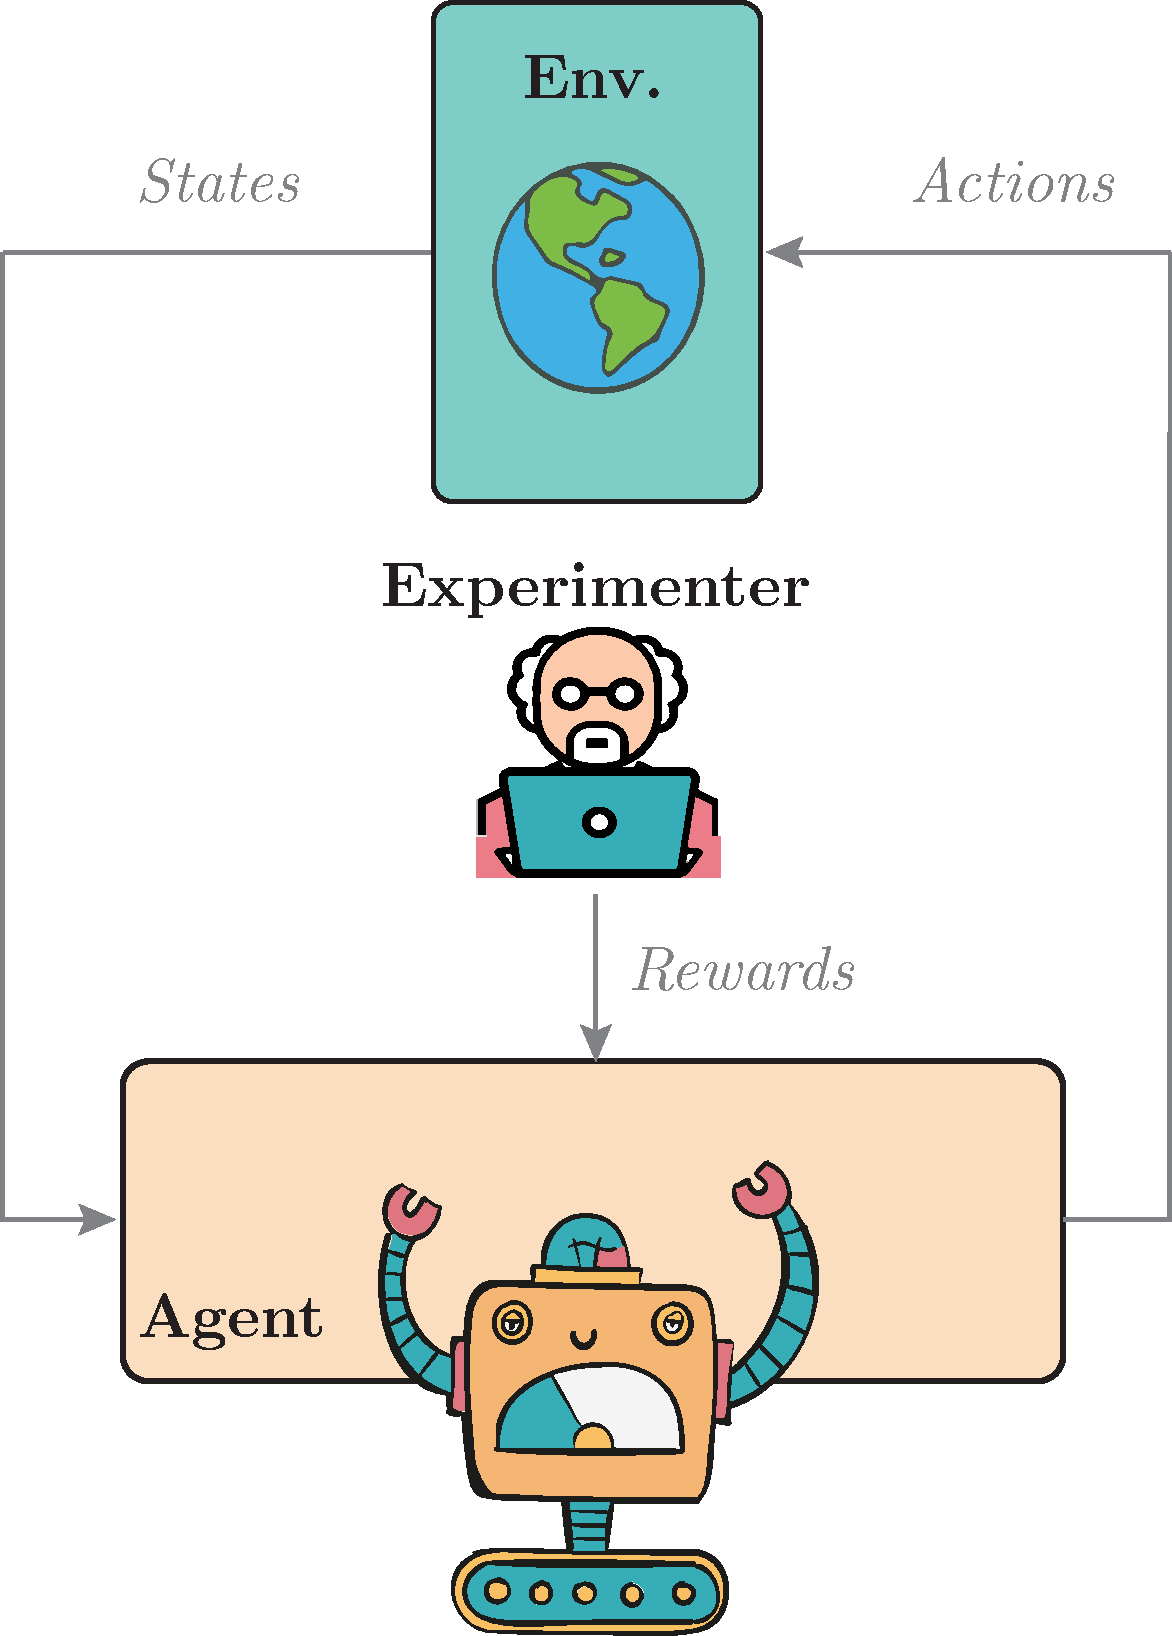
\includegraphics[width=0.3\textwidth]{background/rl_interactions.pdf}	
\caption{}
\label{fig:rl_interacvtions}
\end{figure}

\paragraph{Solution}

The \rl problem can be tackled by several types of optimization methods. In this survey, we focus on \rl
algorithms, as they currently demonstrate stronger capacities in multi-goal problems \cite{goalgan,eysenbach2018diversity,warde2018unsupervised,pong2019skew,lynch2020grounding,hill_human_2020,hill_grounded_2020,abramson_imitating_2020,imagine,team2021open}.

\rl algorithms use transitions collected via interactions between the agent and its environment $(s,\,a,\,s',\,R(s,\,a,\,s'))$ to train a \textit{policy} $\pi$: a function generating the next action $a$ based on the current state $s$ so as to maximize a cumulative function of rewards. Deep \rl  (\drl) is the extension of \rl algorithms that leverage deep neural networks as function approximators to represent policies, reward and value functions. It has been powering most recent breakthrough in \rl  \cite{eysenbach2018diversity,warde2018unsupervised,goalgan,pong2019skew,lynch2020grounding,hill_human_2020,hill_grounded_2020,abramson_imitating_2020,imagine,team2021open}.


\subsection{Imitation Learning}

\paragraph{Problem}

\paragraph{Interactions}

\begin{figure}[!h]
\centering
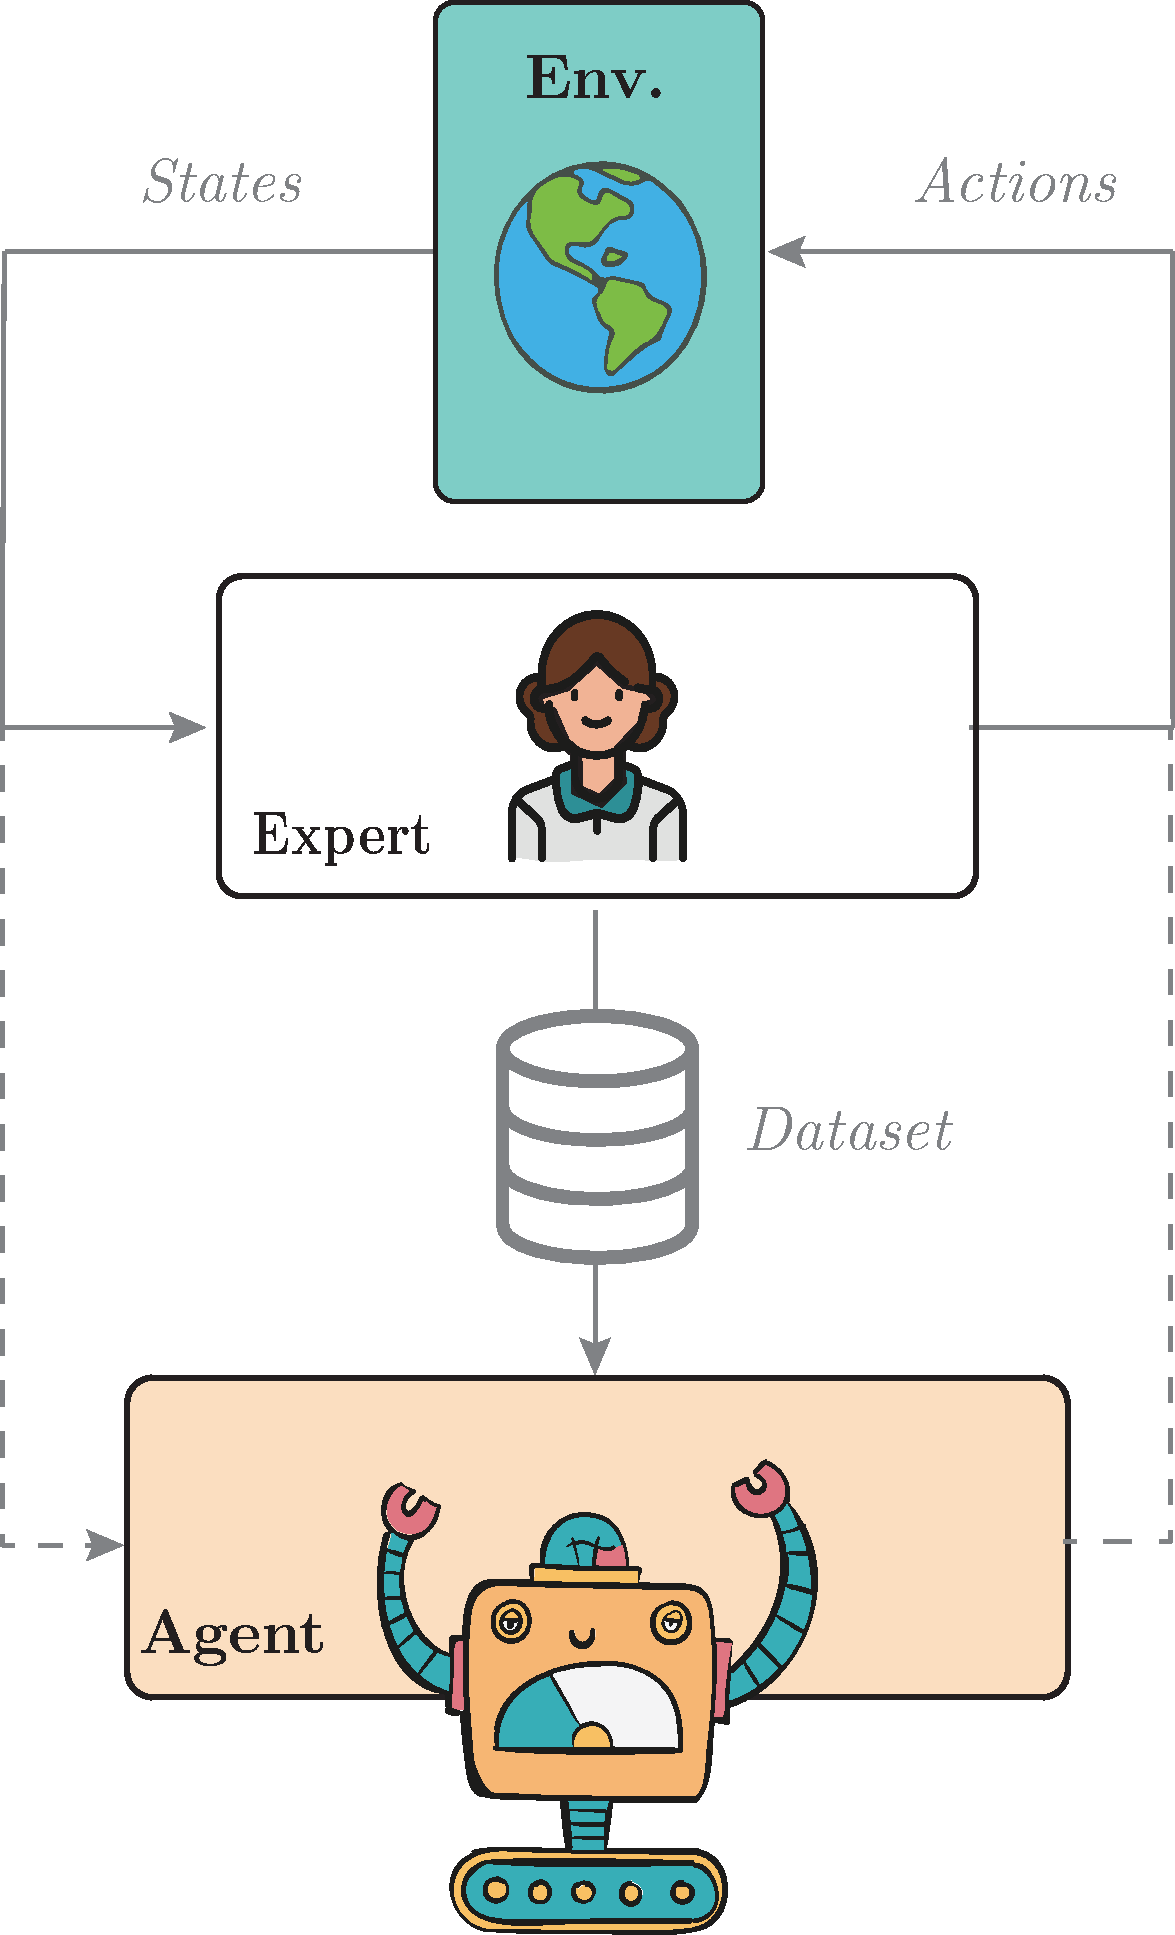
\includegraphics[width=0.3\textwidth]{background/il_interactions.pdf}	
\caption{}
\label{fig:il_interacvtions}
\end{figure}


\paragraph{Solution}

\textbf{Behavioral Cloning}

\textbf{Inverse Reinforcement Learning}

\subsection{Muli-Goal Reinforcement Learning}

\paragraph{Problem}

By replacing the unique reward function $R$ by the space of reward functions $\m{R}_\m{G}$, \rl problems can be extended to handle multiple goals: $\m{M}\,=\,\{\m{S},\,\m{A},\,\m{T},\,\rho_0,\,\m{R}_\m{G}\}$. The term \textit{goal} should not be mistaken for the term \textit{task}, which refers to a particular \mdp instance. As a result, \textit{multi-task} \rl refers to \rl algorithms that tackle a set of \mdps that can differ by any of their components (\eg $\m{T}$,\,$R$,\,$\m{S}_0$, etc.). The \textit{multi-goal} \rl problem can thus be seen as the particular case of the multi-task \rl problem where \mdps differ by their reward functions. In the standard multi-goal \rl problem, the set of goals\,---\,and thus the set of reward functions\,---\,is pre-defined by engineers. The experimenter sets goals to the agent, and provides the associated reward functions. 


\paragraph{Interactions}

\begin{figure}[!h]
\centering
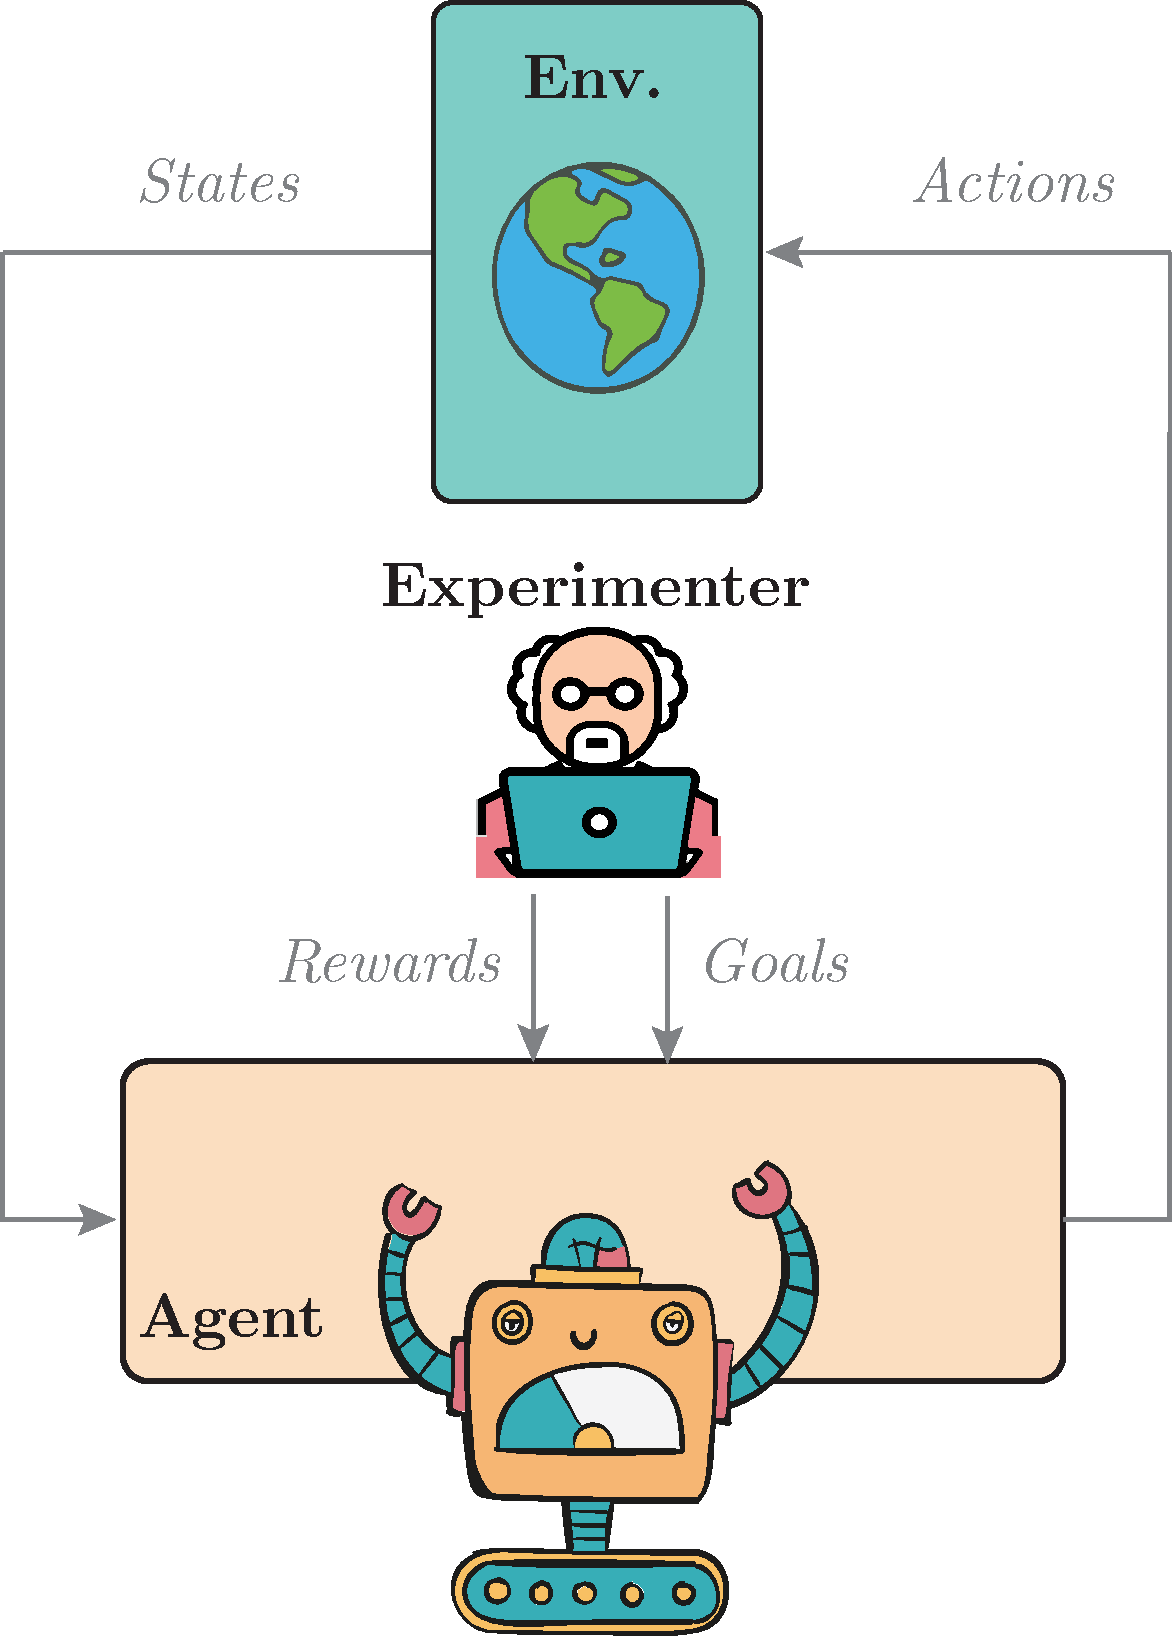
\includegraphics[width=0.3\textwidth]{background/multi_goal_rl_interactions.pdf}	
\caption{}
\label{fig:mg_rl_interacvtions}
\end{figure}


\paragraph{Solution}

Goal-conditioned agents see their behavior affected by the goal they pursue. This is formalized via goal-conditioned policies, that is policies which produce actions based on the environment state and the agent's current goal: $\Pi:\m{S}\times\m{Z}_\m{G}\to\m{A}$, where $\m{Z}_\m{G}$ is the space of goal embeddings corresponding to the goal space $\m{G}$ \cite{schaul2015universal}. Note that ensembles of policies can also be formalized this way, via a meta-policy $\Pi$ that retrieves the particular policy from a one-hot goal embedding $z_g$ \cite{kaelbling1993learning,sutton2011horde}.

The idea of using a unique \rl agent to target multiple goals dates back to \cite{kaelbling1993learning}. Later, the \horde architecture proposed to use interaction experience to update one value function per goal, effectively transferring to all goals the knowledge acquired while aiming at a particular one \cite{sutton2011horde}. In these approaches, one policy is trained for each of the goals and the data collected by one can be used to train others.

Building on these early results, \cite{schaul2015universal} introduced \textit{Universal Value Function Approximators} (\uvfa). They proposed to learn a unique goal-conditioned value function and goal-conditioned policy to replace the set of value functions learned in \horde. Using neural networks as function approximators, they showed that \uvfas enable transfer between goals and demonstrate strong generalization to new goals.

The idea of \textit{hindsight learning} further improves knowledge transfer between goals \cite{kaelbling1993learning,andrychowicz2017hindsight}. Learning by hindsight, agents can reinterpret a past trajectory collected while pursuing a given goal in the light of a new goal. By asking themselves, \textit{what is the goal for which this trajectory is optimal?}, they can use the originally failed trajectory as an informative trajectory to learn about another goal, thus making the most out of every trajectory \cite{eysenbach2020rewriting}. This ability dramatically increases the sample efficiency of goal-conditioned algorithms and is arguably an important driver of the recent interest in goal-conditioned \rl approaches.


\subsection{Multi-Agent Reinforcement Learning}

\paragraph{Problem}

\paragraph{Interactions}

\begin{figure}[!h]
\centering
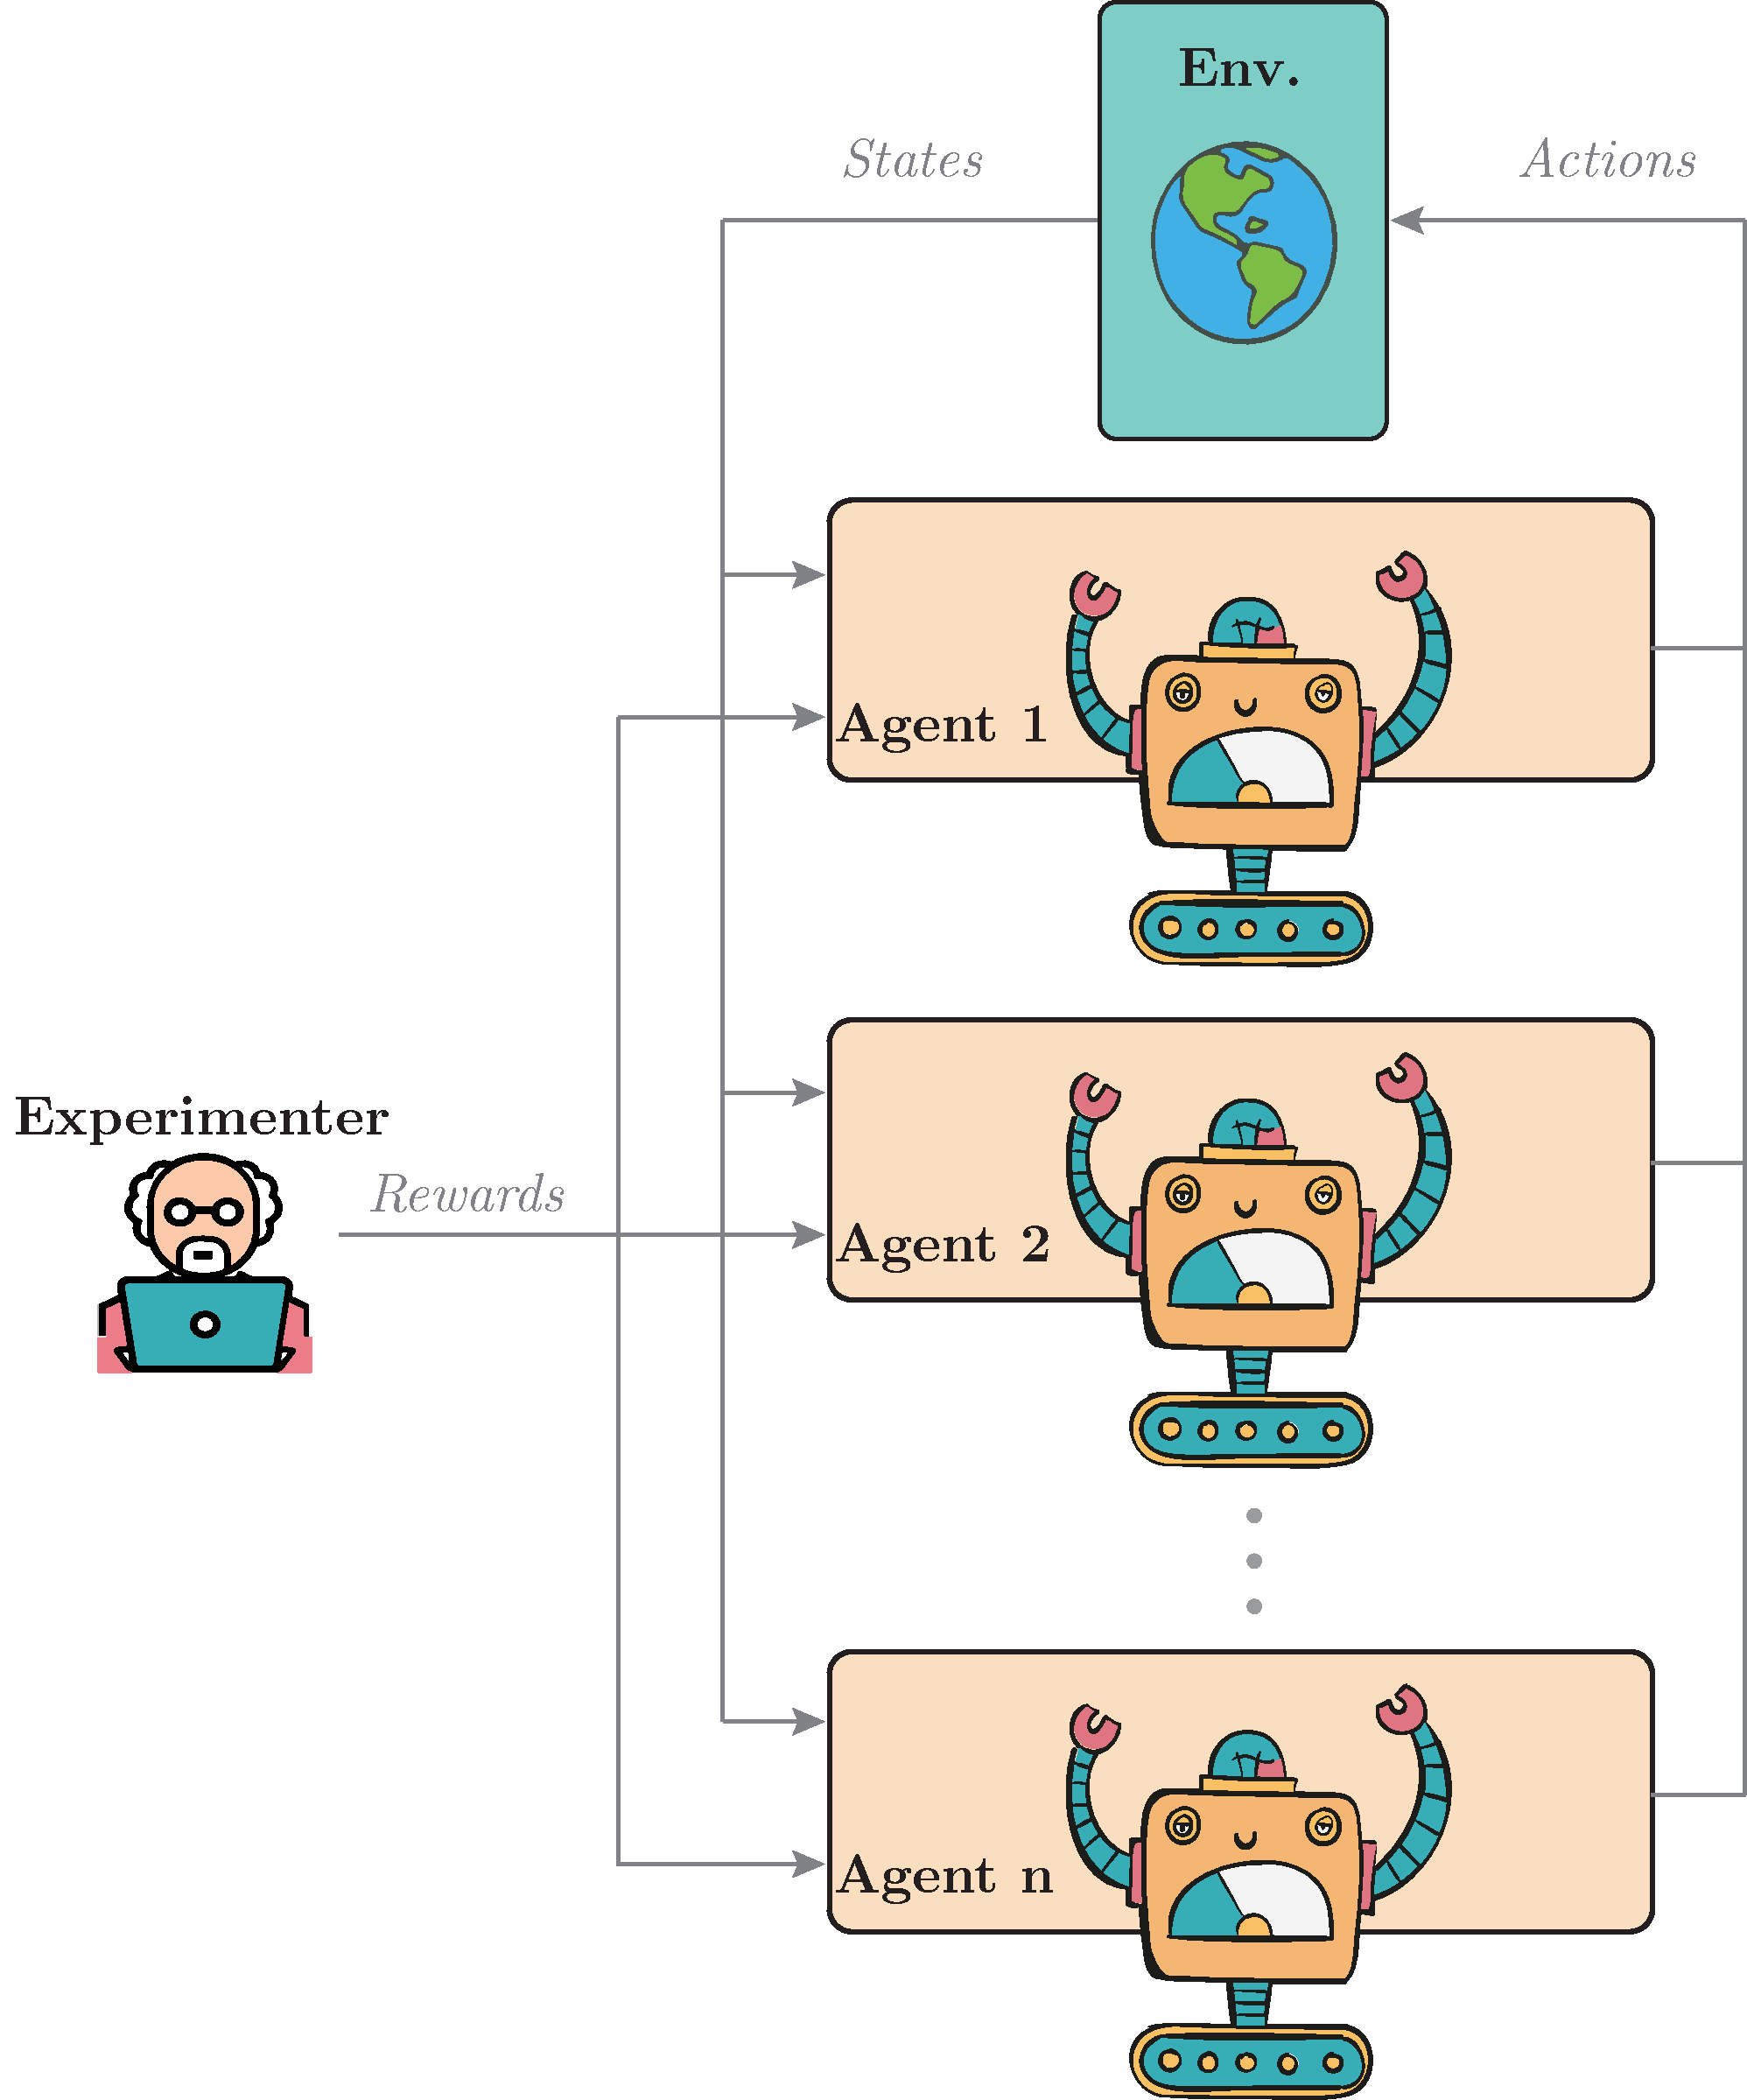
\includegraphics[width=0.5\textwidth]{background/marl_interactions.pdf}	
\caption{}
\label{fig:marl_interacvtions}
\end{figure}


\paragraph{Solution}

\section{Problem Definition: Developmental AI}

\todo{add definition of self-organization}

\subsection{Language Acquisition Problem}


\paragraph{Language Games}

\paragraph{MARL communication}


\subsection{Open-ended Skill Acquisition Problem}



